\nonstopmode
\documentclass[a4paper,UKenglish,cleveref, autoref]{lipics-v2019}

\usepackage{amsmath,amssymb,amsthm,mathtools}
\usepackage[linesnumbered, ruled]{algorithm2e}
\usepackage[final]{microtype}
\usepackage[final]{hyperref}
\usepackage[inline]{enumitem}
\usepackage{subcaption}

% ERR FIX
\usepackage[T1]{fontenc}  


% DEBUG
\usepackage{lipsum}
\usepackage{fullpage}
\usepackage{lineno}
\linenumbers

% EXTRA
\usepackage{authblk}

\tikzset{every picture/.style={
	very thick
% 	,>=Latex
	,>=stealth
}}

% LINES
\tikzset{
	line blue/.style={blue,dotted}
	,line red/.style={red,dashed}
	,line brown/.style={brown,dashdotted}
	,line teal/.style={teal,dashdotdotted}
}

% NODE
\tikzset{default node/.style={
	draw, 
	circle,
	inner sep=0mm,
	minimum size=5mm,
	very thick,
	font=\small
}}

\tikzset{
colored node/.style={line width=1.6pt, star, minimum size=9mm,inner sep=0pt,scale=0.9,}, 
red node/.style={colored node, draw=red, star points=2},
blue node/.style={colored node, draw=blue, star points=3},
green node/.style={colored node, draw=green, star points=4},
black node/.style={colored node, draw=black, star points=5},
orange node/.style={colored node, draw=orange, star points=6},
brown node/.style={colored node, draw=brown, star points=8},
teal node/.style={colored node, draw=teal, star points=10},
violet node/.style={colored node, draw=violet, star points=12},
olive node/.style={colored node, draw=olive, star points=14},
cyan node/.style={colored node, draw=cyan, star points=18},
}

% EDGES
\tikzset{
	light/.style={
		thin,
		gray,
	},
	path/.style={
		light,
		decorate, 
		decoration={snake, segment length=18pt},
	},
	brace/.style={
		decorate,
		decoration={brace, amplitude=5},
		-,
	},
}

\tikzset{e1/.style={cyan}}
\tikzset{e2/.style={green, loosely dash dot dot}}
\tikzset{e3/.style={blue, loosely dotted}}
\tikzset{e4/.style={loosely dashed}}
\tikzset{e5/.style={red, loosely dashed}}
\tikzset{e6/.style={orange, loosely dash dot}}

% LABELS
\tikzset{
	label/.style={
		rectangle,
		draw=none,
		sloped,
		midway,
		fill=white,
		inner sep=2pt,
		minimum height=0,
		minimum width=0,
	},
	label above/.style={
		label,
		above,
	},
	label below/.style={
		label,
		below,
	},
	label inside/.style={
		label,
		fill=white,
		draw=black,
	},
}


% MISC
\tikzset{
	cloud/.style={
		-,
		decorate, 
		decoration={
			snake, 
			segment length=3mm,
			amplitude=.5mm,
		},
	}
	,outline/.style={
		dotted
		,purple
		,very thick	
	}
	,packing/.style={
		outline
		,-
	}
	,m/.style={blue, dashed}
}




\DeclareMathOperator*{\argmin}{arg\,min}
\DeclareMathOperator*{\argmax}{arg\,max}

\def\R{\mathbb{R}}
\def\N{\mathbb{N}}

\newtheorem{observation}{Observation}
\newtheorem{lemma}{Lemma}
\newtheorem{theorem}{Theorem}

\newcommand{\defeq}{\vcentcolon=}

\newcommand\todo[1]{\textcolor{red}{TODO }{#1}}
% \renewcommand\todo[1]{}

\title{A Fast and Simple Algorithm for Submodular Maximization with a Knapsack Constraint}
\titlerunning{A Fast and Simple Algorithm for Submodular Knapsack}

\author{Ariel Kulik}{Department of Computer Science, Technion, Haifa, Israel}{kulik@cs.technion.ac.il}{}{}
\author{Gilad Kutiel}{Department of Computer Science, Technion, Haifa, Israel}{gkutiel@cs.technion.ac.il}{}{}
\author{Roy Schwartz}{Department of Computer Science, Technion, Haifa, Israel}{schwartz@cs.technion.ac.il}{}{}
\authorrunning{A.\,Kulik and G.\,Kutiel and R.\,Schwartz}

\Copyright{Ariel Kulik and Gilad Kutiel and Roy Schwartz}
\ccsdesc{}

%\ccsdesc[100]{ {\color{red}{TBD}} }
%\ccsdesc[100]{ {\color{red}{TBD}} }

\ccsdesc[100]{Theory of computation~Submodular optimization and polymatroids}
\ccsdesc[100]{Theory of computation~Approximation algorithms analysis}

\keywords{knapsack, submodular function, approximation algorithm}

%\category{}

%\relatedversion{}

%\supplement{}

\nolinenumbers



\newcommand{\SK}{{\textsc{Submodular Knapsack}}\xspace}



\begin{document}
\maketitle

\begin{abstract}
We consider the problem of maximizing a monotone submodular function with a knapsack constraint.
In this work we aim at finding fast and simple algorithms for the problem.
Previously, the best fast and simple algorithm is that of Khuller {\em et. al.} [IPL`99] which runs in time $O(n^2)$ and achieves an approximation guarantee of $(1-e^{-\nicefrac[]{1}{2}})\approx 0.393 $.
We present a new fast and simple algorithm which retains the same running time and has an improved approximation guarantee of $0.4536$.
%At the heart of our analysis lies a method that enables us to better analyze the greedy ``bang per buck'' algorithm in the presence of elements with varying cost.
Moreover, we present a general method for ``amplifying'' the approximation factor of any algorithm for the problem, while losing little in the constants of the running time.
Applying this amplification to our new algorithm enables us to further improve the results obtained.
We believe that our amplification method might be of independent interest.

\end{abstract}

\section{Introduction}
In the \emph{Budgeted Maximum Cover} problem we are given a ground set of elements 
$X = \{x_1, \dots, x_n\}$ and a collection of subsets over $X$, 
$\mathcal{S} = \{S_1, \dots, S_m\}$.
A cost function, $c:\mathcal{S} \to \mathbb{R}_+$ assigns cost to each set 
and a weight function $w:X \to \mathbb{R}_+$ assigns weight to each element. 
The goal is to find a collection of sets $\mathcal{S'} \subseteq \mathcal{S}$ such that the 
total cost of the sets in the collection does not exceed a given budget, $B$, and the 
total weight of the elements covered by $\mathcal{S'}$ is maximal.
Khuller et. al \cite{khuller1999budgeted} 
give a $(1-e^{-1})$-approximation algorithm for this problem and show that this
is the best possible unless P = NP.   

A set function $f$ is \emph{submodular} if $f(A \cap B) + f(A \cup B) \leq f(A) + f(B)$ 
for every two sets in the domain of the function. A set function, $f$, is \emph{monotone} if 
$f(A) \leq f(B)$ for every two sets, $A \subseteq B$, in the domain of the function.
Given a set of elements $U = \{e_1, \dots, e_n\}$, a cost function, 
$c:U \to \mathbb{R}_+$ and a monotone, submodular function, $f:2^U \to \mathbb{R}_+$ 
the goal in the \emph{Submodular Function Under
Knapsack Constraint Maximization} problem is to find a subset of $U$ with total cost that does not exceed
a given budget, $B$, with maximal value with respect to $f$.
This problem generalized the \emph{Budgeted Maximum Cover} problem. 
Sviridenko \cite{sviridenko2004note} showed that the same algorithm presented by 
Khuller et. al can be used to maximize general monotone submodular function 
with the same guarantee.
This algorithm requires $O(n^5)$ calls to the value oracle. 

A faster algorithm that runs in $O(n^2)$ time and achieves a $1 - e^{-1/2}$ approximation ratio
was also presented in \cite{khuller1999budgeted}. 
It was shown by Krause and Guestrin \cite{krause2005note} that the same algorithm 
gives that same guarantee for a general monotone submodular function and requires only 
$O(n^2)$ calls to the value oracle.
In the above papers (and other papers as well), however, 
there is a logical flaw in the analysis of this algorithm. 
In this paper we proof this claim. 
We also consider a modification of this algorithm with the same running time and show that it
achieves a better approximation ratio.   

\section{Preliminaries}\label{sec:Preliminaries}
We consider the Submodular Function Under
Knapsack Constraint Maximization problem.
For a given instance we denote by $O$ an optimal solution and for the rest of the 
paper we assume, without loose of generalization, that both the 
given budget and the optimal value are both equal one, that is $B = f(O) = 1$.
We also assume, without loose of generalization, 
that the cost function is in the range $[0, 1]$.
 
If it is clear from the context we use $x$ to denote the set $\{x\}$. 
We use the notation $f(B|A)$ to denote $f(A \cup B) - f(A)$, that is the marginal value of $B$
given $A$. 
For a set of elements, $A$, we use $c(A)$ to denote $\sum_{e \in A}c(e)$.
For an ordered set $A = \{a_1, \dots, a_k\}$ we use $A_i$ to denote the subset 
$\{a_i, \dots, a_i\}$, $A_0$ denote the empty set. 

The greedy algorithm from \cite{khuller1999budgeted} and \cite{krause2005note}
is described in Algorithm \ref{alg:greedy}.

\begin{algorithm}[H]
\label{alg:greedy}

\SetKwInOut{Input}{input}
\SetKwInOut{Output}{output}

\Input{$U = \{e_1, \dots, e_n\}$, $f:2^U\to \mathbb{R}_+$, $c:U \to \mathbb{R}_+$}
\Output{$S \subseteq U$}

initialization: $S \leftarrow \emptyset$
\\
\While{$U \neq \emptyset$}{
	$e' \leftarrow \displaystyle{\arg\max_{e \in U}}\frac{f(e|S)}{c(e)}$
	\\
	$U \leftarrow U \setminus e'$
	\\
	\If{$c(S \cup \{e'\})\leq 1$}{
	\label{line:dropped}
		$S \leftarrow S \cup \{e'\}$
	}
}
\Return{S}
\caption{Greedy Algorithm}
\end{algorithm}
 
If the condition in line \ref{line:dropped} is evaluated to false we say that the algorithm 
\emph{dropped} the element $e'$.
It can be shown that, in the worse case, the performance of the greedy algorithm 
can be arbitrarily bad.

Let $S$ be the output of the greedy algorithm, the \emph{Modified Greedy} algorithm 
returns the best among the output of the greedy algorithm
and the best singleton, that is $\arg\max\{S, \displaystyle{\arg\max_{e \in U}}f(\{e\})\}$,
Algorithm~\ref{alg:mgreedy} depicts this algorithm.  

\begin{algorithm}[H]
\label{alg:mgreedy}

\SetKwInOut{Input}{input}
\SetKwInOut{Output}{output}

\Input{$U = \{e_1, \dots, e_n\}$, $f:2^U\to \mathbb{R}_+$, $c:U \to \mathbb{R}_+$}
\Output{$S \subseteq U$}

$S \leftarrow \text{greedy}(U, f, c)$
\\
\Return{$\arg\max\{S, \displaystyle{\arg\max_{e \in U}}f(\{e\})\}$}
\caption{Modified Greedy Algorithm}
\end{algorithm}

We also consider in this paper the \emph{modified modified greedy} algorithm~\ref{alg:mmgreedy}

\begin{algorithm}[H]
\label{alg:mmgreedy}

\SetKwInOut{Input}{input}
\SetKwInOut{Output}{output}

\Input{$U = \{e_1, \dots, e_n\}$, $f:2^U\to \mathbb{R}_+$, $c:U \to \mathbb{R}_+$}
\Output{$S \subseteq U$}

$S \leftarrow \text{greedy}(U, f, c)$
\\
\Return{$\arg\max\{S, \displaystyle{\arg\max_{e_1, e_2 \in U}}f(\{e_1, e_2\})\}$}
\caption{Modified Modified Greedy Algorithm}
\end{algorithm}

The following lemma plays an important roll in the rest of this paper.

\begin{lemma}
\label{lemma:main}
Let $A = \{a_1, \dots, a_k\}$ and $B$ be two subsets such that for all $1 \leq i \leq k$ 
and for all $e \in B$ it holds that 
$\frac{f(a_i|A_{i-1})}{c(a_i)} \geq \frac{f(e|A_{i-1})}{c(e)}$
then $f(A) \geq (1 - e^{-\frac{c(A)}{c(B)})}f(B)$.
\end{lemma} 

\begin{proof}
\todo{proof}.
\end{proof}


\todo{rephrase}
In particular, Lemma~\ref{lemma:main} can be applied on a set of consecutive 
elements picked by the greedy algorithm and compare their value...   






\section{Correct Proof for Approximation Factor of Modified Greedy}\label{sec:ModifiedGreedy}
Let $O$ be an optimal set and recall that we assume that $f(O) = 1$.
Let $T = \arg\max\{S, \displaystyle{\arg\max_{e \in U}}f(\{e\})\}$ 
be the set returned by the modified greedy algorithm, 
where $S$ is the set computed by the greedy algorithm~\ref{alg:greedy},
we prove the following theorem:

\begin{theorem}
$f(T) \geq (1 - e^{-1/2})$.
\end{theorem}

\begin{proof}
We can assume that $f(e) \leq 1 - e^{-1/2}$ for every $e \in U$ or otherwise the proof holds. 
Note, also, that if $|O \setminus T| \leq 1$ then $f(T) \geq 0.5$. 
Thus we assume the algorithm drops at least two elements from $O$ during its running. 
Denote by $x$ and $y$ the first and second such elements respectively.
Denote by $A$ the set of elements chosen by the algorithm just before dropping $x$ and by
$B$ the set of elements chosen right after dropping $x$ and before dropping $y$.
If $f(A) \geq 1 - e^{-1/2}$ the theorem holds, otherwise denote $f(A) = 1 - e^{-(1/2 - \delta)}$,
where $\delta$ might be in the range $(0, 0.5)$.  

We argue that the following inequalities hold:

\begin{align}
c(A) \leq 0.5 - \delta 
\\
c(x) > 0.5 + \delta
\\
c(O \setminus x) \leq 0.5 - \delta
\\
c(B) > 2\delta
\\
f(x) < 1 - e^{-1/2}
\\
\label{ineq:T}
f(O \setminus x | A) \geq e^{-1/2} - 1 + e^{-(1/2 - \delta)}
\\
\label{ineq:B}
f(B|A) \geq (1 - e^{-\frac{2\delta}{1/2 - \delta}})f(O \setminus x | A)
\\
f(T) \geq f(A) + f(B|A)
\end{align}

\todo{explain the inequalities}.

Substituting $f(A) = 1 - e^{-(1/2 - \delta)}$ 
and $f(B|A) \geq (1 - e^{-\frac{2\delta}{1/2 - \delta}})f(O \setminus x | A)$
into the last inequality gives the desired result as can be seen in Figure~\ref{fig:mgreedy}
\end{proof}

\begin{figure}
\caption{
\label{fig:mgreedy}
Modified Greedy Approximation Ratio
}
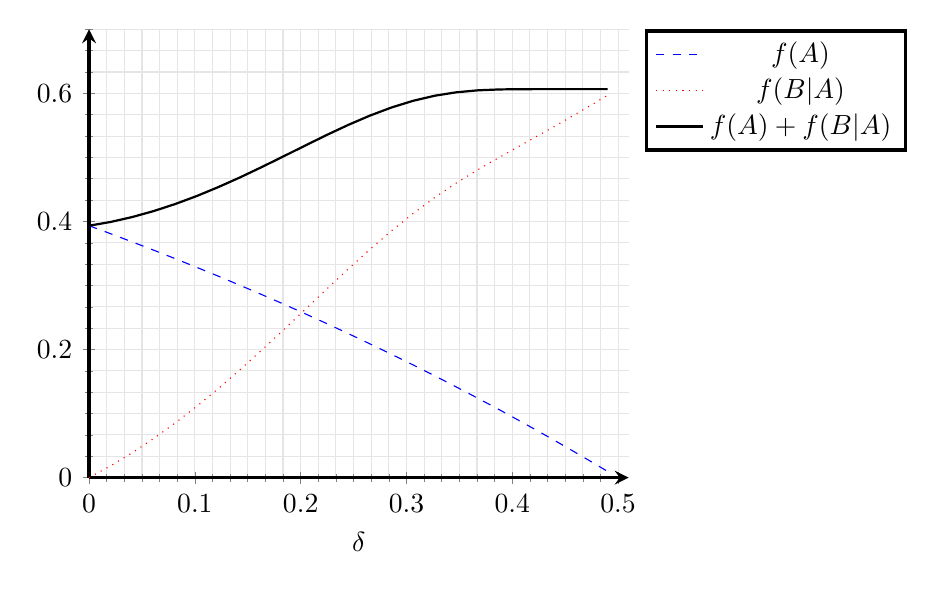
\begin{tikzpicture}
\begin{axis}[
	domain=0:0.49
	,ymax=.7
	,xmax=.51
	,xlabel=$\delta$
	,axis lines=left
	,grid=both
	,grid style={
		draw=gray!20
	}
	,minor tick num=5
	,legend pos=outer north east
	,legend entries={
		$f(A)$
		,$f(B|A)$
		,$f(A) + f(B|A)$
	}
]
  \addplot[blue, dashed, thin]{1-exp(-(0.5-x))};
  \addplot[red, dotted, thin]{(1 - exp(-(4*x/(1-2*x)))) * (exp(-1/2) - 1 + exp(-(1/2-x)))};
  \addplot[black, thick]{1-exp(-(0.5-x)) + (1 - exp(-(4*x/(1-2*x)))) * (exp(-1/2) - 1 + exp(-(1/2-x)))};
\end{axis}
\end{tikzpicture}
\end{figure}



\section{The Modified\textsuperscript{2} Greedy Algorithm}\label{sec:Modified2Greedy}
We now analyze the modified modified greedy algorithm.

Let $\epsilon > 0$ a constant to be determined latter on, and let $T$ be the output of 
the algorithm.

\begin{theorem}
$f(S) \geq 1 - e^{-(1/2 + \epsilon)}$
\end{theorem}

\begin{proof}
We can assume that $f(\{e_1, e_2\}) \leq 1 - e^{-1/2 + \epsilon}$ 
for every $e_1, e_2 \in U$ or otherwise the proof holds.
Note, also, that if $|O \setminus T| \leq 2$ then $f(T) \geq 0.5$.
Thus we assume the algorithm drops at least three elements from $O$ during its running.
Let $x$ be the first element in $O$ that was dropped by the algorithm, 
and let $A$ be the set of elements chosen by the algorithm just before dropping $x$.
If $f(A) \geq 1 - e^{-1/2}$ the theorem holds, 
otherwise denote $f(A) = 1 - e^{-(1/2 + \epsilon - \delta)}$.
We say that an element, $e$, is \emph{expensive} if $c(e) \ge 1/4 + \epsilon/2 - \delta/2$, 
otherwise it is \emph{cheap}.
Observe that $O$ contains at most two expensive elements, thus the algorithm drops 
at least one cheap element from $O$. 
Let $y$ be the first such element, and let $B$ be the set of elements chosen by the 
algorithm right after dropping $x$ and just before dropping $y$.
Also denote by $C$ the subset of cheap elements in $O$, 
i.e. $C = \{e \in O : c(e) < 1/4 + \epsilon/2 - \delta/2\}$.

We argue that the following inequalities hold:

\begin{align}
c(A) \leq 0.5 + \epsilon - \delta 
\\
c(x) > 0.5 -\epsilon + \delta
\\
c(C) \leq 0.5 + \epsilon - \delta
\\
c(B) > 2\delta
\\
f(C) \ge e^{-1/2 + \epsilon}
\\
c(B) \ge 1/4 - 3\epsilon/2 + 3\delta/2
\\
f(B|A) \ge \left[
e^{-(1/2 + \epsilon)}
- (1 - e^{-(1/2 + \epsilon - \delta)})
\right]
(1-e^{-\frac{1-6\epsilon+6\delta}{2+4\epsilon-4\delta}})
\\
f(T) \geq \max_\epsilon \min \{1 - e^{-(0.5 + \epsilon)}, \min_{\delta} f(A) + f(B|A)\}
\end{align}
\todo{explain the inequalities}.

Substituting $f(A) = 1 - e^{-(1/2 - \delta)}$ into the last inequality, 
using $f(B|A) \ge \left[
e^{-(1/2 + \epsilon)}
- (1 - e^{-(1/2 + \epsilon - \delta)})
\right]
(1-e^{-\frac{1-6\epsilon+6\delta}{2+4\epsilon-4\delta}})
$,
and setting (say) $\epsilon = 0.104$ gives the desired result 
as can be seen in Figure~\ref{fig:mmgreedy}.

\end{proof}

\begin{figure}
\def\eps{0.104}
\caption{
\label{fig:mmgreedy}
Modified Modified Greedy Approximation Ratio ($\epsilon = 0.104$)
}
\begin{tikzpicture}
\begin{axis}[
	width=\textwidth
	,domain=0:0.49
	,ymax=.7
	,xmax=.51
	,xlabel=$\delta$
	,xtick distance=0.1
	,ytick distance=0.1
	,axis lines=left
	,grid=both
	,grid style={
		draw=gray!20
	}
	,minor tick num=5
	,legend pos=south west
	,legend entries={
		$f(A)$
		,$f(B|A)$
		,$f(A) + f(B|A)$
	}
]
  \addplot[blue, dashed, thin]{1-exp(-(0.5 + \eps -x))};
  \addplot[red, dotted, thin]{
  	(1 - exp(-(1 - 6 * \eps + 6 * x)/(2 + 4 * \eps - 4 * x)))
  	*
  	(exp(-(0.5 + \eps) - 1 + exp(-(0.5 + \eps - x))))
  };
  \addplot[black, thick]{
  	1-exp(-(0.5 + \eps -x))
  	+
  	(1 - exp(-(1 - 6 * \eps + 6 * x)/(2 + 4 * \eps - 4 * x)))
  	*
  	(exp(-(0.5 + \eps) - 1 + exp(-(0.5 + \eps - x))))
  };
\end{axis}
\end{tikzpicture}
\end{figure}

\paragraph{Upper Bound}
We show that the approximation ratio of the modified modified greedy algorithm is at most $0.5$.
To see this consider the following instance of the budgeted maximum coverage problem:
Let the elements be $X = \{x_1, \dots, x_{2n}\}$, 
and a collection of subsets over $X$, $\mathcal{S} = \{S_1, \dots, S_{n + 1}\} \cup \{S\}$,
where for each $1 \leq i \leq n + 1$, $S_i = \{x_i\}$, and $c(S_i) = 1$. 
Also, set $S = \{x_{n + 2}, \dots, x_{2n}\}$, and $c(S) = n$.
Finally, for each $x \in X$ set $w(x) = 1$ and set the budget for this instance to be $2n$.
One can verify that the modified modified algorithm will return a solution of value $n + 1$
While taking $S$ along with any other $n$ subsets yields a solution of value $2n - 1$.  





\section{Amplification Algorithm}\label{sec:Amplification}
\def\pLarge{P_{\text{large}}}
\def\pVal{P_{\text{val}}}
\def\MGreedy{Modified$^2$Greedy}
\def\BOTAlg{BestOfThree}
\def\mA{\mathcal{A}}

In this section we show a simple algorithm, which given
an $r$-approximation $\mA$ for \SK, $r<1/2$ can
be used to derive an $r'$-approximation, $r<r' <1/2$, for
\SK using  a constant number of calls
for $\mA$ and $\frac{3n^2}{2}+n$ oracle queries.

Algorithm \ref{algorithm:amplify} receives
an approximation algorithm $\mA$ for $\SK$,ƒo
a universe $U$, a monotone non-negative
submodular function $f:2^U \rightarrow \mathbb{R}$,
a non-negative cost function $c:U \rightarrow \mathbb{R}$, and a budget $\beta$.
The algorithm also gets two scalar parameters $\epsilon$
and $\rho$.  These two parameters control the approximation
ratio and complexity of the algorithm, and should be set according
to the claims in this section to obtain the required approximation
ratio and complexity.

Broadly speaking,  the algorithm finds the pair of  elements with maximal value $\pVal$. It then divides all pairs of elements $\{a,b\} \subseteq U$ for which
$\frac{f(\{a,b\})}{f(\pVal)} \geq \rho$ into {\em buckets}, where the subsets
in each bucket have the same value to a factor of $(1+\epsilon)$.
The algorithm then extends the set of smallest cost in  each bucket
to a solution using the algorithm $\mA$.  The algorithm returns the
best between the solutions found using the buckets and $\mA$, the pair of
elements with maximal profit, the single element with maximal profit, and the result of the greedy algorithm
over the input instance.

\begin{algorithm}
	\caption{Amplify($\mA, U, f, c, \beta, \epsilon, \rho$)}
	\label{algorithm:amplify}
	% Initialization
	\tcp{Initialization}
	$\pVal \leftarrow \argmax_{ \{a,b\} \subseteq U, c(\{a,b\})\leq \beta } f(\{a,b\})$
	\\ $w_{\max}\leftarrow f(\pVal)$
	\\ $i_{\max} \leftarrow \floor{\log_{1 + \epsilon} \frac{1}{\rho}}$
	\\
	\tcp{Buckets}
	\For{$i \in \{0,\dots,i_{\max}\}$}{
		$B_i = \left\{ \{a,b\}\subseteq U| c(\{a,b\})\leq \beta, \rho(1+\epsilon)^i \leq \frac{f(\{a,b\})}{w_{\max}}  < \rho (1+\epsilon)^{i+1} \right\}$
		\\
		$P_i \leftarrow \argmin_{\{a,b\}\in B_i} c(\{a,b\})$
%	}
%	\tcp{Candidate Solutions}
%	\For{$i \in \{0,\dots,i_{\max}\}$}{
\\
		$S_i \leftarrow P_i \cup \mA(U , f_{P_i}, c, \beta - c(P_i))$
	}
	$G \leftarrow \text{Greedy}(U, f, c, \beta)$ \label{amplify:greedy}
	\\
	$T \leftarrow \argmax_{\{a\}\subseteq U| c(a)\leq \beta} f(\{a\})$ \label{amplify:singletons}
	\\
	\Return $\argmax_{S \in \{S_0, S_1, \ldots, S_{i_{\max}}, G, \pVal,T\}} f(S)$
	%

\end{algorithm}

The following function, which already appeared on Theorem \ref{thrm:Amplification}, will be useful throughout the analysis of the algorithm:

$$ B(\alpha)=1-e^{-\frac{1}{\alpha}}$$
$$ A(\alpha) = \frac{1}{1-e^{-\alpha}}-\frac{1}{B(\alpha)}$$
 $$D(\alpha)=(1-e^{-\alpha})/B(\alpha)$$

 \begin{lemma}
 	\label{lemma:amplification}
 	Given an $r$-approximation $\mA$ for $\SK$ where $r<\frac{1}{2}$.
 	For any $0< \alpha \leq  \ln 2$, input $U,f,c,\beta$ of $\SK$,
 	and $\epsilon$ such that $0<\epsilon\leq \frac{1-2r}{r}$, then executing
 	Algorithm \ref{algorithm:amplify}  with parameters
 	$(\mA, U, f, c, \beta, \epsilon, A(\alpha))$ returns
 	$$min\left(1-e^{-\alpha}, D(\alpha) + (1-r) \left( \frac{2+\epsilon}{1+\epsilon}(1- D(\alpha)) -1 \right) \right)$$
 	approximation for the input instance.
 \end{lemma}



\begin{proof}

	Fix an optimal solution $O$.
	 If $|O|\leq 2$ the algorithm returns an optimal solution and the Lemma holds.
	Therefore we can assume $|O| \geq 3$.  Denote by $\pLarge$ the set of  two  elements in $O$ with highest cost.
	
	Let $L\beta$ be the highest cost of element in $O$.  If $L\leq 1-\alpha$ then
	by Lemma \ref{lemma:sub-main} and the monotonicity of $f$: $f(G) \geq (1-e^{-\alpha}) f(O)$  (recall that $G$ is the result of
	greedy in line \ref{amplify:greedy} of the algorithm and thus Lemma \ref{lemma:sub-main} can be applied on the appropriate prefix of $G$). Therefore, the algorithm
	returns a solution of value at least $(1-e^{-\alpha})f(O)$ and the Lemma holds. Therefore we can assume  $L> 1-\alpha$.
%
%	{\color{red}
%	consider $G'\subseteq G$ to be the subset selected by the greedy (in line \ref{amplify:greedy})
%	just before the first element from $O$ has been dropped ($G' = G$ if no such element exists).
%	Due to the greedy procedure selection of elements the conditions of Lemma \ref{lemma:sub-main}
%	hold for $G'$ (as $A$)  and $O$ (as $B$), therefore,
%}  $f(G) \geq (1-e^{-\alpha}) f(O)$. Therefore, the algorithm
%	returns a solution of value at least $(1-e^{-\alpha})f(O)$ and the Lemma holds. Hence, we can assume  $L> 1-\alpha$.
	
	If $O\setminus \pLarge \subseteq G$, then
	$f(G)+ f(\pVal)\geq f(O\setminus \pLarge) + f(\pLarge) \geq f(O)$.
	Therefore $f(G)\geq \frac{f(O)}{2}$ or $f(\pVal)\geq \frac{f(O)}{2}$
	thus the Lemma holds (note that $\alpha \leq ln 2$ and therefore
	$1-e^{-\alpha} < \frac{1}{2}$). Thus we can assume that
	$O\setminus \pLarge \nsubseteq G$.
	
	The following corollary states that if $f(\pLarge)$ is fairly small
	with respect to $f(O)$ (equivalently, $f(O|\pLarge)$ is high) then the solution $G$ from the greedy algorithm provides
	the required approximation ratio.
	
	\begin{corollary}
		\label{corollary:cor1}
	If $f(O|\pLarge) \geq D(\alpha) f(O)$ then $f(G)\geq (1-e^{-\alpha})f(O)$.
	\end{corollary}

\begin{proof}
	

	Let $\beta M$ be the third highest cost of element in  $O$.
	As the highest cost of  element in $O$ is $\beta L$,
	using a simple argument we get, $M\leq M(L)$ where $M(L)= \min \{\frac{1-L}{2}, L\}$. Since
	$O\setminus \pLarge \nsubseteq G$, there must be an element from $O \setminus \pLarge$ the greedy in line \ref{amplify:greedy} drops. Since all the elements
	in $O\setminus \pLarge$ are of cost at most $\beta M$ the knapsack must
	already have elements of cost $\beta (1-M)$ at the first time an element from $O\setminus \pLarge$ is dropped. Also, $c(O\setminus \pLarge) \leq \beta(1-L -M)$, therefore by Lemma \ref{lemma:sub-main} and the monotonicity of $f$ we get that:
  	$$f(G)\geq \left(1-e^{- \frac{\beta (1-M) }{c(O\setminus \pLarge)}}\right) f(O\setminus \pLarge)
  			\geq \left(1-e^{- \frac{1-M }{1-L-M}}\right) f(O\setminus \pLarge) .$$
  			
  	We note that the term $\frac{1-M}{1-L-M} = \left(  1- \frac{L}{1-M} \right)^{-1}$ is increasing as a function
  	of $M$  in the range $[0, M(L)]$ (note that $1-L-M >0$ in the range).
  	Therefore $\frac{1-M}{1-L-M} \geq  \frac{1 }{1-L}  \geq \frac{1}{1-(1-\alpha)} = \nicefrac[]{1}{\alpha}$. And conclude
  %	The term  $1-e^{- \frac{1-M(L) }{1-L-M(L)}}$ is increasing as a function of $L$
  %	({\bf this is not trivial, I simply drew the graph on Desmos for that}), therefore
  	%	as $L> (1-\alpha)$ we get
  %		$$f(G)\geq  \left(1-e^{- \frac{1-M(L) }{1-L-M(L)}}\right) f(O\setminus \pLarge)
  	%	\geq \ \left(1-e^{- \frac{1-M(1-\alpha) }{1-(1-\alpha)-M(1-\alpha)}}\right) f(O\setminus \pLarge) $$
  		
  	%As $\frac{2}{3} \leq \alpha \leq \ln 2$ we have $M(1-\alpha) = 1-\alpha$. Combining this with the previous inequality we get
  	  $$f(G)
  	\geq \ \left(1-e^{- \frac{1-M }{1-L-M}}\right) f(O\setminus \pLarge) \geq \left( 1- e ^ {- \frac{1}{ \alpha}} \right)f(O\setminus \pLarge)
  	= B(\alpha)f(O\setminus \pLarge) $$
  	
  	Now, recall that $D(\alpha)= \frac{1-e^{-\alpha}}{B(\alpha)}$,
	$f(O|\pLarge) \geq D(\alpha) f(O)$ by the condition of the
	lemma and $f(O|\pLarge) \leq f(O\setminus \pLarge)$ as
	$f$ is submodular. Using these observations and the last lower
	bound on $f(G)$ we obtain
%	\begin{equation*}
%\begin{array}{rcl}
\begin{align*}
f(G) \geq& B(\alpha)f(O\setminus \pLarge)  \geq
B(\alpha) f(O|\pLarge)\\  \geq&
B(\alpha ) D(\alpha ) f(O)
= B(\alpha)\frac{1-e^{-\alpha}}{B(\alpha) }f(O)= (1-e^{-\alpha})f(O)
\end{align*}
%\end{array}
%	\end{equation*}

	\end{proof}

	\begin{corollary}
		\label{corollary:cor2}
		If $f(G)< (1-e^{-\alpha})f(O)$ and $f(\pVal) < (1-e^{-\alpha})f(O)$ then
		$f(\pLarge) \geq A(\alpha) f(\pVal)$
		\end{corollary}
	\begin{proof}
		As $f(G)< (1-e^{-\alpha})$, the condition of corollary \ref{corollary:cor1} does not hold. Therefore
		$f(O|\pLarge)< D(\alpha) f(O)$. Hence,
		$$f(O)= f(\pLarge) + f(O|\pLarge) < f(\pLarge) + D(\alpha) f(O)$$
		By rearranging the terms and using $f(\pVal) < (1-e^{-\alpha})f(O)$
		we get
		$$f(\pLarge) > (1-D(\alpha)) f(O) > \frac{1-D(\alpha)}{1-e^{-\alpha}} f(\pVal)
		= \left(\frac{1}{1-e^{-\alpha}} - \frac{D(\alpha)}{1-e^{-\alpha}}\right) f(\pVal) = A(\alpha) f(\pVal)$$
		The second inequality uses the observation that $D(\alpha) \leq 1$ for $0\leq \alpha \leq 1$ which can be easily verified. The last equality follows from the definitions
		of $D(\alpha)$ and $A(\alpha)$.
		
			
		\end{proof}

	\begin{corollary}
		\label{corollary:cor3}
			If $f(G)< (1-e^{-\alpha})f(O)$ and $f(\pVal) < (1-e^{-\alpha})f(O)$ then
			there is $i\in \{0, \ldots, i_{\max}\}$ such that
		$$\frac{f(S_i)}{f(O)} \geq D(\alpha) + (1-r)\left( \frac{2+\epsilon}{1+\epsilon} D(\alpha) -1 \right)$$
	\end{corollary}
\begin{proof}
		As the conditions of corollary \ref{corollary:cor2} hold, we have
		$f(\pLarge) \geq A(\alpha) f(\pVal)$.
		 Let $i$ be the minimal integer $i$ such
		that $\frac{f(\pLarge)}{f(\pVal)} < A(\alpha)(1+\epsilon) ^{i+1}$, as $f(\pLarge) \geq A(\alpha) f(\pVal)$ we get $i\geq 0$.
		Recall that $i_{\max}= \floor{\log_{1+\epsilon} \frac{1}{\rho} } =
		\floor{\log_{1+\epsilon} \frac{1}{A(\alpha)}} $ (as the algorithm is used
			with $\rho=A(\alpha)$).
			Therefore,
			$$A(\alpha) (1+\epsilon) ^{i_{\max} +1}
			> A(\alpha) \frac{1}{A(\alpha) } = 1 \geq \frac{f(\pLarge)}{f(\pVal)}$$
			Thus $i\leq i_{\max}$.
			Also $c(\pLarge) \leq c(O) \leq \beta$, and we can conclude that
			$\pLarge \in B_i$ (note that $w_{\max} = f(\pVal)$).
			
			From the definition of $P_i$ we get $c(P_i)\leq c(\pLarge)$ and
			$f(P_i) \geq \frac{1}{1+\epsilon} f(\pLarge)$.
			Let $Q_i  =  \mA(U, f_{P_i}, c, \beta - c(P_i))$.
			As $c(P_i) \leq c(\pLarge)$ we get that $O\setminus \pLarge$
			is a feasible solution for the problem instance given to $\mA$.
			Hence, as $\mA$ is a $r$-approximation we get
			$$f(Q_i | P_i) \geq r f(O\setminus \pLarge| P_i)$$
			Therefore,
			\begin{align*}
			f(S_{i})
			&
			\geq f(P_i) + f(Q_i|P_i)
			\\ &
			\geq f(P_i) + r f(O \setminus \pLarge | P_i)
			\\ &
			\geq f(P_i) + r(f(O) - f(\pLarge) - f(P_i))
			\\ &
			= (1-r)f(P_i) + r(f(O) - f(\pLarge))
			\\ &
			\geq \frac{1-r}{1 + \epsilon}f(\pLarge) + r(f(O) - f(\pLarge))
			\\ &
			= \left(
			\frac{(2 + \epsilon)}{(1 + \epsilon)}(1-r) - 1
			\right)
			f(\pLarge)
			+ rf(O)
			\label{eq:sub:bucket}
			\end{align*}
			
			As $\epsilon\leq \frac{1-2r}{r}$ one can deduce that
			$\left(
			\frac{(2 + \epsilon)}{(1 + \epsilon)}(1-r) - 1
			\right) \geq 0$.
			Also, since $f(G)< (1-e^{-\alpha})f(O)$ by corollary \ref{corollary:cor1} we
			get $f(O|\pLarge)  <D(\alpha)f(O)$, by using $f(O|\pLarge)= f(O) -f(\pLarge)$
			and rearranging  the terms we get
			$f(\pLarge)> (1-D(\alpha)) f(O)$.
			Therefore,
			\begin{align*}
			f(S_i) \geq&
			\left(
			\frac{(2 + \epsilon)}{(1 + \epsilon)}(1-r) - 1
			\right)
			f(\pLarge)
			+ rf(O) \\ \geq &
				\left(
			\frac{(2 + \epsilon)}{(1 + \epsilon)}(1-r) - 1
			\right) (1-D(\alpha ) )f(O) +rf(O)\\
			=& f(O) \left(  D(\alpha) + (1-r)\left(  \frac{(2 + \epsilon)}{(1 + \epsilon)} (1-D(\alpha)) -1\right) \right)
			\end{align*}
			and the corollary immediately follows.
			
		
	\end{proof}
The Lemma follows immediately from corollary \ref{corollary:cor3} as it states
that either $G$, $\pVal$ or $S_i$ for some $i$ would provide the required approximation
ratio.
\end{proof}

\begin{lemma}
	\label{lemma:amp_runtime}
Algorithm \ref{algorithm:amplify} uses $\floor{\log_{1+\epsilon} \frac{1}{\rho}}+1$
	invocation to $\mA$ and up to $\frac{3}{2} n ^2+n$ additional oracle queries.
 \end{lemma}
\begin{proof}
	The number of invocation to $\mA$ immediately follows from the algorithm.
	Beside the invocation to $\mA$ the algorithm runs the greedy procedure
	which uses up to $n^2$ queries. The queries for the initialization and
	buckets phases only considers sets of size $2$, and therefore can be
	implemented by up to $n(n-1)/2\leq n^2/2$ queries. The execution
	of line \ref{amplify:singletons} would take another $n$ queries.
	\end{proof}



\begin{proof}[Proof of Theorem \ref{thrm:Amplification}]
	Let $$\alpha^*  = \argmax _{0<\alpha \leq \ln{2}} \left\{ \min \left\{ 1-e^{-\alpha},D(\alpha)+(1-r)\left( \frac{2+\nu(\alpha)}{1+\nu(\alpha)} (1-D(\alpha)) -1\right)\right\}\right\}$$
	We obtain the described approximation ratio when running the algorithm
	with $\epsilon = \nu(\alpha^*)$ and $\rho = A(\alpha^*)$.
	By the conditions of the theorem,
	$$k \geq -\frac{\log A(\ln 2)} { \log(\nicefrac[]{1}{r} -1 ) } +1 \geq-\frac{\log A(\alpha*)} { \log(\nicefrac[]{1}{r} -1 ) } +1 $$
	Where the last inequality uses the fact that $A$ is monotonically decreasing.  Thus,
	$$\epsilon^* = 2 ^{-\frac{\log_2 (A(\alpha^*))}{k-1}} -1 \leq \
	2 ^{-\frac{ \log_2(A(\alpha^*))}{  -\left(\frac{\log_2(A(\alpha* ))}{\log_2(\nicefrac[]{1}{r}-1)} \right) }} -1  =
	2^{\log_2(\nicefrac[]{1}{r}-1)} -1 = \nicefrac[]{1}{r}-2 = \frac{1-2r}{r} $$
	therefore the conditions of Lemma \ref{lemma:amplification} apply,
	and the approximation ratio follows.
	
	By lemma \ref{lemma:amp_runtime} the number of invocations for $\mA$
	is
	\begin{align*}
	\floor{\log_{1+\epsilon^*} \frac{1}{A(\alpha^*)}}+1 \leq \
	-\log_{1+\epsilon^*} (A(\alpha^*)) +1 =
	\frac{-\log A(\alpha^*)} {\log(1+\epsilon^*)} +1 \\
	= \frac{-\log {A(\alpha^*)}} {\log(2 ^{-\frac{\log_2 (A(\alpha^*))}{k-1}} )} +1
	= \frac{-\log {A(\alpha^*)}} {-\frac{\log_2 (A(\alpha^*))}{k-1}} +1
	= k \end{align*}
	and the number of addition oracle queries is $\nicefrac[]{3n^2}{2} + n $
	as required.
	
\end{proof}

 

\bibliographystyle{plainurl}
\bibliography{main}

\appendix
\section{Omitted Proofs}
\label{appendix:omitted}
\begin{proof}[Proof of Lemma \ref{lemma:sub-main}]
	

		Consider $a_i$ and observe that:
		\begin{align}
		\frac{f(a_i|A_{i-1})}{c(a_i)}c(B)
		& = \sum_{e \in B} \frac{f(a_i|A_{i-1})}{c(a_i)}c(e)
		\nonumber
		\\ 	& \geq \sum_{e \in B} \frac{f(e|A_{i-1})}{c(e)}c(e)
		\label{ineq:main:cond}
		\\	& \geq f(B|A_{i-1})
		\label{ineq:main:sub}
		\\ 	& \geq f(B) - f(A_{i-1}).
		\label{ineq:main:mon}
		\end{align}
		Inequality \eqref{ineq:main:cond} follows from the condition in the lemma, inequality \eqref{ineq:main:sub} follows from the submodularity of $f$, and inequality \eqref{ineq:main:mon} follows from the monotonicity of $f$.
		Thus, from the above we can conclude that:
		$$
		f(B) - f(A_i)  \leq (f(B) - f(A_{i - 1}))
		\left(1 - \frac{c(a_i)}{c(B)}\right).
		$$
		Hence,
		$$
		f(B) - f(A_i)  \leq f(B) \prod_{j = 1}^{i}
		\left(1 - \frac{c(a_j)}{c(B)}\right).
		$$
		Applying the inequality $1 - x \leq e^{-x}$ we get that:
		$$
		f(B) - f(A_i)  \leq f(B)\cdot
		e^{-\frac{c(A_i)}{c(B)}}.
		$$
		Rearranging the terms and setting $i = k$ completes the proof.

	
	
	
\end{proof}





\end{document}
